% +------------------------------------------------------------------------+
% | CGAL Reference Manual:  hds.tex
% +------------------------------------------------------------------------+
% | Combinatoric and geometry of polyhedral surfaces in 
% | halfedge representation.
% |
% | 11.10.1996   Lutz Kettner
% |              Start rewriting the whole stuff
% | 
\RCSdef{\hdsRev}{$Revision$}
\RCSdefDate{\hdsDate}{$Date$}
% +------------------------------------------------------------------------+

\ccParDims

\chapter{Halfedge Data Structures}
\label{chapterHalfedgeDS}
\ccChapterRelease{\hdsRev. \ \hdsDate}\\
\ccChapterAuthor{Lutz Kettner}


% +------------------------------------------------------------------------+
\section{Introduction}

A halfedge data structure (abbreviated as \ccc{HalfedgeDS}, or
\ccc{HDS} for template parameters) is an edge-centered data structure
capable of maintaining incidence informations of vertices, edges and
faces, for example for planar maps, polyhedra, or other orientable,
two-dimensional surfaces embedded in arbitrary dimension. Each edge is
decomposed into two halfedges with opposite orientations. One incident
face and one incident vertex are stored in each halfedge.  For each
face and each vertex one incident halfedge is stored.  Reduced
variants of the halfedge data structure can omit some of these
informations, for example the halfedge pointers in faces or the
storage of faces at all.

\begin{ccTexOnly}
    \vspace{-4mm}
    \begin{center}
      \parbox{0.4\textwidth}{%
          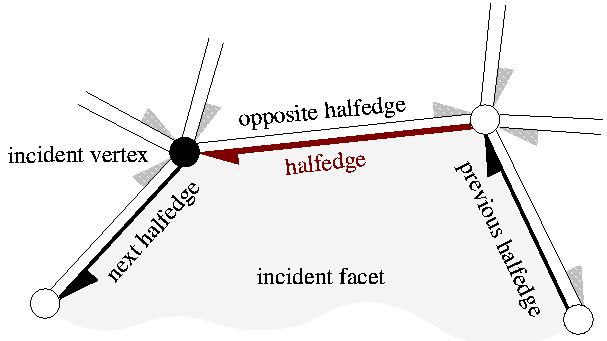
\includegraphics[width=0.4\textwidth]{fig/halfedge.ips}%
      }
    \end{center}
    \vspace{-3mm}
\end{ccTexOnly}

\begin{ccHtmlOnly}
    <CENTER>
    <A HREF="./halfedge.gif">
        <img src="./halfedge_small.gif" alt="Halfedge Diagram"></A><P>
    </CENTER>
\end{ccHtmlOnly}

The halfedge data structure is a combinatorial data structure,
geometric interpretation is added by classes built on top of the
halfedge data structure.  These classes might be more convenient to
use than the halfedge data structure directly, since the halfedge data
structure is meant as an implementation layer.  See for example the
\ccc{CGAL::Polyhedron_3} class in Chapter~\ref{chapterPolyhedron}
and Chapter~\ref{chapterPolyhedronRef}.

The data structure provided here is also known as the
FE-structure~\cite{w-ebdss-85}, as
halfedges~\cite{m-ism-88,bfh-mgedm-95} or as the doubly connected edge
list (DCEL)~\cite{bkos-cgaa-97}, although the original reference for
the DCEL~\cite{mp-fitcp-78} describes a different data structure. The
halfedge data structure can also be seen as one of the variants of the
quad-edge data structure~\cite{gs-pmgsc-85} that supports only
orientable 2-manifolds. In general, the quad-edge data structure can
represent also non-orientable 2-manifolds.  An overview and comparison
of these different data structures together with a thorough
description of the design implemented here can be found
in~\cite{k-ugpdd-99}.  The design presented here is a revised and
incompatible version of the previous design~\cite{k-ddsps-98} as used
in \cgal\ R2.1 and earlier releases.

% +------------------------------------------------------------------------+
\section{Software Design}


\begin{ccTexOnly}
  \begin{figure}
    \begin{center}
      \parbox{0.7\textwidth}{%
          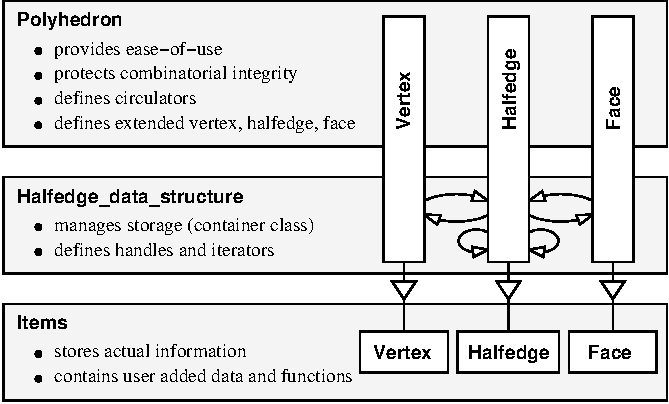
\includegraphics[width=0.7\textwidth]{fig/hds_design.ips}%
      }
    \end{center}
    \caption{Responsibilities of the different layers in the 
             halfedge data-structure design.}
    \label{figureHalfedgeDSDesign}
  \end{figure}
\end{ccTexOnly}

\begin{ccHtmlOnly}
    <CENTER>
    <A NAME="figureHalfedgeDSDesign">
        <img src="./hds_design_col.gif"
         alt="Halfedge Data-Structure Design"><BR>
    Figure: Responsibilities of the different layers in the 
            halfedge data-structure design.
    <P>
    </CENTER>
\end{ccHtmlOnly}

Figure~\ccTexHtml{\ref{figureHalfedgeDSDesign}}{}\begin{ccHtmlOnly}
  <A HREF="Chapter_main.html#figureHalfedgeDSDesign"><IMG 
  SRC="cc_ref_up_arrow.gif" ALT="reference arrow" WIDTH="10" HEIGHT="10"></A>
\end{ccHtmlOnly}
illustrates the responsibilities of the three layers of the software
design with the \ccc{CGAL::Polyhedron_3} as an example for the top
layer.  The items provide the space for the information that is
actually stored, i.e.~with member variables and access member
functions in \ccc{Vertex}, \ccc{Halfedge}, and \ccc{Face}
respectively. Halfedges are required to provide a reference to the
next halfedge and to the opposite halfedge.  Optionally they may
provide a reference to the previous halfedge, to the incident vertex
and to the incident face. Vertices and faces may be empty. Optionally
they may provide a reference to the incident halfedge. The options
mentioned are supported in the halfedge data structure and the
polyhedron, for example Euler operations update the optional
references if they are present. Furthermore, the item classes can be
extended with arbitrary attributes and member functions, which will be
promoted by inheritance to the actual classes used for the polyhedron.

Vertices, halfedges and faces are passed as local types of the
\ccc{Items} class to the halfedge data structure and polyhedron.
Implementations for vertices, halfedges and faces are provided that
fulfill the mandatory part of the requirements. They can be used as
base classes for extensions by the user. Richer implementations are
also provided to serve as defaults; for polyhedra they provide all
optional incidences, a three-dimensional point in the vertex type and
a plane equation in the face type.

The \ccc{Halfedge_data_structure} is responsible of the storage
organization of the items. Currently, implementations using internally
a bidirectional list or an \stl\ vector are provided. The
\ccc{Halfedge_data_structure} defines the handles and iterators
belonging to the items. These types are promoted to the declaration of
the items themselves and are used there to provide the references to
the incident items. This promotion of types is done with a template
parameter \ccc{Refs} of the item types.  The halfedge data structure
provides member functions to insert and delete items, to traverse all
items, and it gives access to the items in order to manipulate the
items.

There are already three different models for the
\ccc{Halfedge_data_structure} available. Therefore we have kept their
interface small. Functionality common to all these models is separated
into a helper class \ccc{Halfedge_data_structure_decorator}, which is
not shown in 
Figure~\ccTexHtml{\ref{figureHalfedgeDSDesign}}{}\begin{ccHtmlOnly}
  <A HREF="Chapter_main.html#figureHalfedgeDSDesign"><IMG 
  SRC="cc_ref_up_arrow.gif" ALT="reference arrow" WIDTH="10" HEIGHT="10"></A>
\end{ccHtmlOnly}, but would be placed at the
side of the \ccc{Halfedge_data_structure} since it broadens that
interface but does not hide it.  This helper class contains operations
that are useful to implement the operations in the next layer, for
example the polyhedron. It adds for example the Euler operations and
partial operations from which further Euler operations can be built
from, such as inserting an edge into the ring of edges at a vertex.
Furthermore, the helper class contains adaptive functionality.  For
example if the \ccc{prev()} member function is not provided for
halfedges, the \ccc{find_prev()} member function of the helper class
searches in the positive direction along the face for the previous
halfedge. But if the \ccc{prev()} member function is provided, the
\ccc{find_prev()} member function simply calls it. This distinction
is resolved at compile time with a technique called {\em
  compile-time tags}, similar to iterator tags in~\cite{sl-stl-95}.

The \ccc{Polyhedron} as an example for the third layer adds the
geometric interpretation, provides an easy-to-use interface of
high-level functions, and unifies the access to the flexibility
provided underneath.  It renames face to facet, which is more common
for three-dimensional surfaces.  The interface is designed to protect
the integrity of the internal representation, the handles stored in
the items can no longer directly be written by the user.  The
polyhedron adds the convenient and efficient circulators, see
Chapter~\ref{chapterCirculators}, for accessing the circular sequence
of edges around a vertex or around a facet. To achieve this, the
\ccc{Polyhedron} derives new vertices, halfedges and facets from those
provided in \ccc{Items}.  These new items are those actually used in
the \ccc{Halfedge_data_structure}, which gives us the coherent type
structure in this design, especially if compared to our previous
design.


% +========================================================================+
\clearpage
\section{Example Programs}
% +========================================================================+
\label{sectionHdsExamples}


% +-------------------------------------------------------------+
\subsection{The Default Halfedge Data Structure}

The following example program uses the default halfedge data structure
and the decorator class. The default halfedge data structure uses a
list based representation. All incidences of the items and a point
type for vertices are defined. The program creates a loop, consisting
of two halfedges, one vertex and two faces, and checks its validity.

\ccIncludeExampleCode{HalfedgeDS/hds_prog_default.C}


% +-------------------------------------------------------------+
\subsection{A Minimal Halfedge Data Structure}

The following program defines a minimal halfedge data structure using
the minimal items class \ccc{CGAL::HalfedgeDS_min_items} and a
list-based halfedge data structure. The result is a data structure
maintaining only halfedges with next and opposite pointers.  No
vertices or faces are stored. The data structure represents an {\em
  undirected graph}.

\ccIncludeExampleCode{HalfedgeDS/hds_prog_graph.C}


% +-------------------------------------------------------------+
\subsection{The Default with a Vector Instead of a List}

The default halfedge data structure uses a list internally and the
maximal base classes. Assuming we have a point type {\tt Point} we
define a halfedge data structure using the same items class but the
vector-based representation.  Note that for the vector storage the
size of the halfedge data structure must be reserved beforehand,
either with the constructor as shown in the example or with the {\tt
  reserve()} member function.

\ccIncludeExampleCode{HalfedgeDS/hds_prog_vector.C}


% +-------------------------------------------------------------+
\subsection{Example Adding Color to Faces}

This example re-uses the base class available for faces and adds a
member variable \ccc{color}.

\ccIncludeExampleCode{HalfedgeDS/hds_prog_color.C}

% +-------------------------------------------------------------+
\subsection{Example Defining a More Compact Halfedge}

\begin{ccAdvanced}
  
The halfedge data structure as presented here is slightly less space
efficient as for example the winged-edge data
structure~\cite{b-prcv-75}, the DCEL~\cite{mp-fitcp-78} or variants of
the quad-edge data structure~\cite{gs-pmgsc-85}.  On the other side,
it does not require any search operations during traversals. A
comparison can be found in~\cite{k-ugpdd-99}.

The following example trades traversal time for a compact storage
representation using traditional C techniques (i.e.~type casting and
the assumption that pointers, especially those from {\tt malloc} or
{\tt new}, point to even addresses). The idea goes as follows: The
halfedge data structure allocates halfedges pairwise.  Concerning the
vector based data structure this implies that the absolute value of
the difference between a halfedge and its opposite halfedge is always
one with respect to C pointer arithmetic. We can replace the opposite
pointer by a single bit encoding the sign of this difference.  We will
store this bit as the least significant bit in the next halfedge
handle.  This example omits the previous pointer. What remains are
three pointers per halfedge. The same solution can be applied to the
list-based halfedge data structure
\ccc{CGAL::HalfedgeDS_using_in_place_list} with the difference that the
{\tt SIZE} constant must reflect the size increase due to the
additional pointers needed for the list management. See 
\texttt{examples/HalfedgeDS/hds\_prog\_compact2.C} for this modified example
program. The list-based halfedge data structure
\ccc{CGAL::HalfedgeDS_using_list} cannot be used since the pairwise
allocation of halfedges is here not guaranteed to happen in
consecutive memory locations. Here is the example for the vector based
data structure.

\ccIncludeExampleCode{HalfedgeDS/hds_prog_compact.C}

\end{ccAdvanced}

% +-------------------------------------------------------------+
\subsection{Example Using the Halfedge Iterator}

Two edges are created in the default halfedge data structure.
The halfedge iterator is used to count the halfedges.

\ccIncludeExampleCode{HalfedgeDS/hds_prog_halfedge_iterator.C}

% +-------------------------------------------------------------+
\subsection{Example for an Adapter to Build an Edge Iterator}

Three edges are created in the default halfedge data structure.
The adapter {\tt N\_step\_adaptor} is used to declare an edge
iterator, which is used to count the edges.

\ccIncludeExampleCode{HalfedgeDS/hds_prog_edge_iterator.C}

% +--------------------------------------------------------+

% =============================================================================
% The CGAL Reference Manual
% Chapter: Optimisation
% -----------------------------------------------------------------------------
% file  : doc_tex/basic/Optimisation/main.tex
% author: Bernd G�rtner, Sven Sch�nherr (sven@inf.fu-berlin.de)
% -----------------------------------------------------------------------------
% $Revision$
% $Date$
% =============================================================================

\newcommand{\linebreakByHand}{\ccTexHtml{\\}{}}
\newcommand{\SaveSpaceByHand}{}  %%%% [2]{\ccTexHtml{#1}{#2}}

\chapter{Geometric Optimisation} \label{Optimisation}
\RCSdefDate{\OptRCSDate}{$Date$}

\ccChapterRelease{Release: 2.0 \ccTexHtml{\quad}{ , } \OptRCSDate}

\ccChapterAuthor{Bernd G{\"a}rtner}\ccTexHtml{\\}{<br>}
\ccChapterAuthor{Michael Hoffmann}\ccTexHtml{\\}{<br>}
\ccChapterAuthor{Sven Sch{\"o}nherr}

\ccTexHtml{\thispagestyle{empty}}{}

\begin{ccTexOnly}\section*{Introduction}\end{ccTexOnly}
\begin{ccHtmlOnly}<H2>Introduction</H2><P>\end{ccHtmlOnly}

This chapter describes routines for solving geometric optimisation problems.
The first two sections contain algorithms for computing and updating the
smallest enclosing circle (Section~\ref{sec:smallest_enclosing_circles})
resp.\ ellipse (Section~\ref{sec:smallest_enclosing_ellipses}) of a finite
point set.  Formally, the `smallest enclosing circle' is the boundary of the
closed disk of minimum area covering the point set. It is known that this
disk is unique.  We usually identify the disk with its bounding circle,
allowing us to talk about points being on the boundary of the circle, etc.
The same holds for the smallest enclosing ellipse. These algorithms work in
an incremental manner. They are implemented as semi-dynamic data structures,
thus allowing to insert points while maintaining the smallest enclosing
circle resp.\ ellipse.

The remaining sections describe algorithms for searching in matrices with
specific properties and some applications. In particular, there are
general implementations of
\begin{itemize}
  \item monotone matrix search (see Section~\ref{secMonotoneMatrixSearch}),
    which can be applied to compute
    \begin{itemize}
      \item extremal polygons of a convex polygon
        (see Section~\ref{secComputingExtremalPolygons}) \textit{or}
      \item all furthest neighbors for the vertices of a convex polygon
        (see Section~\ref{secAllFurthestNeighbors}),
    \end{itemize}
  \item and sorted matrix search (see Section~\ref{secSortedMatrixSearch}),
    which can be used to compute the $p$-centers of a planar point set
    (see Section~\ref{sec_RectangularPCenters}).
\end{itemize}

\subsubsection*{Traits Class}
The class and function templates are parameterized with a traits class
which defines the abstract interface between the optimisation
algorithm and the primitives it uses. We provide traits class
implementations that interface the optimisation algorithms with the
\cgal\ kernel. For some algorithms, in addition, we provide traits
class adapters to user supplied point classes. Finally, we describe
the requirements that must be fulfilled by traits classes for
optimisation algorithms.  This is at the same time a specification for
using the provided traits class implementations as for users who want
to supply their own traits class.

\subsubsection*{Assertions}
The optimisation code uses infix \ccc{OPTIMISATION} in the assertions,
e.g.\ defining the compiler flag
\ccc{CGAL_OPTIMISATION_NO_PRECONDITIONS} switches precondition
checking off, cf.~Section~\ref{assertions}.

\newcommand{\cgalSetOptTraitsAdaptLayout}{\ccTexHtml{%
    \ccSetThreeColumns{CGAL_Oriented_side}{}{returns constants
      \ccc{CGAL_LEFTTURN}, \ccc{CGAL_COLLINEAR}}
    \ccPropagateThreeToTwoColumns}{}}
\newcommand{\cgalSetOptTraitsAdaptReqLayout}{\ccTexHtml{%
    \ccSetThreeColumns{CGAL_Oriented_side}{da.get_hw( Point p).}{}
    \ccPropagateThreeToTwoColumns}{}}

\newcommand{\cgalSetOptTraitsReqLayout}{\ccTexHtml{%
    \ccSetThreeColumns{CGAL_Oriented_side}{}{returns
      \ccc{CGAL_ON_BOUNDED_SIDE}, \ccc{CGAL_ON_BOUNDARY}}
    \ccPropagateThreeToTwoColumns}{}}

\ccHtmlNoClassToc

\input{smallest_enclosing_circles}

\input{smallest_enclosing_ellipses}

%% ==============================================================
%% Specification: Computing Extremal Polygons
%% --------------------------------------------------------------
%% file  : spec_extremal_polygons.awi
%% author: Michael Hoffmann
%% $Id$
%% ==============================================================

\clearpage
\section{Computing Extremal Polygons}
\label{secComputingExtremalPolygons}
\cgalColumnLayout

This section describes several functions to compute a maximal $k$-gon
$P_k$ that can be inscribed into a given convex polygon $P$. The
criterion for maximality can be chosen freely by defining an
appropriate traits class as specified in section
\ref{req_ExtremalPolygonTraits}. For \cgal\ point classes there are
two predefined traits classes to compute a maximum area (see section
\ref{secMaximumAreaInscribedKgon}) resp.  perimeter (see section
\ref{secMaximumPerimeterInscribedKgon}) inscribed $k$-gon.

\ccHtmlNoClassToc
\begin{ccHtmlClassFile}{computing_maximum_area_inscribed_k_gon.html}
  {Function Declaration of \ccc{maximum_area_inscribed_k_gon}}
  \ccHtmlNoClassIndex\ccHtmlNoClassLinks
  %% class wrapper to keep the font at a uniform size:
  \begin{ccClass}{dummy}
    \ccHtmlNoIndex\subsection{Computing a Maximum Area Inscribed $k$-gon}
  \label{secMaximumAreaInscribedKgon}
  \end{ccClass}
  
  This section describes a function to compute a maximal area $k$-gon
  $P_k$ that can be inscribed into a given convex polygon $P$. Note
  that $P_k$ is not unique in general, but it can be chosen in such a
  way that its vertices form a subset of the vertex set of $P$.

  \ccInclude{CGAL/extremal_polygon_2.h}

  \def\ccLongParamLayout{\ccTrue} 
  
  \ccGlobalFunction{
    template < class RandomAccessIC, class OutputIterator >
    OutputIterator
    maximum_area_inscribed_k_gon(
    RandomAccessIC points_begin,
    RandomAccessIC points_end,
    int k,
    OutputIterator o);}
  
  computes a maximum area inscribed $k$-gon of the convex polygon
  described by [\ccc{points_begin}, \ccc{points_end}), writes its
  vertices to \ccc{o} and returns the past-the-end iterator of this
  sequence.
  
  \ccHeading{Precondition}
  \begin{enumerate}
  \item Value type of \ccc{RandomAccessIC} has to be
    \ccc{Point_2<R>} for some representation class \ccc{R}.
  \item \ccc{OutputIterator} accepts the value type of
    \ccc{RandomAccessIC} as value type,
  \item the -- at least three -- points denoted by the range
    [\ccc{points_begin}, \ccc{points_end}) form the boundary of a convex
    polygon (oriented clock-- or counterclockwise) \textit{and}
  \item $k \ge 3$.
  \end{enumerate}

  \ccHeading{Note}
  
  On compilers not supporting member function templates, the parameter
  \ccc{RandomAccessIC} is fixed to \ccc{vector<Point_2>::iterator}
  where \ccc{Point_2} is the value type of \ccc{RandomAccessIC}.
  
  \ccImplementation The implementation uses monotone matrix
  search\cite{akmsw-gamsa-87} and has a worst case running time of $O(k
  \cdot n + n \cdot \log n)$, where $n$ is the number of vertices in
  $P$.

  \ccExample The following code generates a random convex polygon
  \ccc{p} with ten vertices and computes the maximum area inscribed
  five-gon of \ccc{p}.

  \ccIncludeVerbatim{extremal_polygon_2_example_area.C}

\end{ccHtmlClassFile}
    
\ccHtmlNoClassToc
\begin{ccHtmlClassFile}{computing_maximum_perimeter_inscribed_k_gon.html}
  {Function Declaration of \ccc{maximum_perimeter_inscribed_k_gon}}
  \ccHtmlNoClassIndex\ccHtmlNoClassLinks
  %% class wrapper to keep the font at a uniform size:
  \begin{ccClass}{dummy}
    \ccHtmlNoIndex\subsection{Computing a Maximum Perimeter Inscribed
      $k$-gon}
    \label{secMaximumPerimeterInscribedKgon}
  \end{ccClass}
  
  This section describes a function to compute a largest perimeter
  $k$-gon $P_k$ that can be inscribed in a given convex polygon $P$.
  Note that $P_k$ is not unique in general, but we know that its
  vertices form a subset of the vertex set of $P$.

  \ccInclude{CGAL/extremal_polygon_2.h}

  \def\ccLongParamLayout{\ccTrue}
  \ccGlobalFunction{
    template < class RandomAccessIC, class OutputIterator >
    OutputIterator
    maximum_perimeter_inscribed_k_gon(
    RandomAccessIC points_begin,
    RandomAccessIC points_end,
    int k,
    OutputIterator o);}
  
  computes a maximum perimeter inscribed $k$-gon of the convex polygon
  described by [\ccc{points_begin}, \ccc{points_end}), writes its
  vertices to \ccc{o} and returns the past-the-end iterator of this
  sequence.

  \ccHeading{Precondition}
  \begin{enumerate}
  \item Value type of \ccc{RandomAccessIC} has to be
    \ccc{Point_2<R>} for some representation class \ccc{R},
  \item there is a global function \ccc{R::FT sqrt( R::FT)}
    defined that computes the squareroot of a number,
  \item \ccc{OutputIterator} accepts the value type of
    \ccc{RandomAccessIC} as value type,
  \item the -- at least three -- points denoted by the range
    [\ccc{points_begin}, \ccc{points_end}) form the boundary of a
    convex polygon (oriented clock-- or counterclockwise) \textit{and}
  \item $k \ge 2$.
  \end{enumerate}

  \ccTagDefaults

  \ccHeading{Note}
  
  On compilers not supporting member function templates, the parameter
  \ccc{RandomAccessIC} is fixed to \ccc{vector<Point_2>::iterator}
  where \ccc{Point_2} is the value type of \ccc{RandomAccessIC}.
  
  \ccImplementation The implementation uses monotone matrix
  search\cite{akmsw-gamsa-87} and has a worst case running time of $O(k
  \cdot n + n \cdot \log n)$, where $n$ is the number of vertices in
  $P$.

  \ccExample The following code generates a random convex polygon
  \ccc{p} with ten vertices and computes the maximum perimeter inscribed
  five-gon of \ccc{p}.

  \ccIncludeVerbatim{extremal_polygon_2_example_perimeter.C}

\end{ccHtmlClassFile}

\begin{ccAdvanced}
  \ccHtmlNoClassToc
  \begin{ccHtmlClassFile}{computing_general_extremal_polygons.html}
    {Function Declaration of \ccc{extremal_polygon}}
    \ccHtmlNoClassIndex\ccHtmlNoClassLinks
    %% class wrapper to keep the font at a uniform size:
    \begin{ccClass}{dummy}
      \ccHtmlNoIndex\subsection{Computing General Extremal
        Polygons}\label{secGeneralExtremalPolygons}
    \end{ccClass}
    
    This section describes a general function to compute a maximal
    $k$-gon $P_k$ that can be inscribed in a given convex polygon $P$.
    The criterion for maximality and some basic operations have to
    specified in an appropriate traits class as specified in section
    \ref{req_ExtremalPolygonTraits}.
    
    \ccInclude{CGAL/extremal_polygons_2.h}

    \def\ccLongParamLayout{\ccTrue} 
    
    \ccGlobalFunction{
      template < class RandomAccessIC, class OutputIterator, class Traits >
      OutputIterator
      extremal_polygon(
      RandomAccessIC points_begin,
      RandomAccessIC points_end,
      int k,
      OutputIterator o,
      const Traits& t);}
    
    computes a maximal (as specified by \ccc{t}) inscribed $k$-gon of
    the convex polygon described by [\ccc{points_begin},
    \ccc{points_end}), writes its vertices to \ccc{o} and returns the
    past-the-end iterator of this sequence.
    
    \ccHeading{Precondition}
    \begin{enumerate}
    \item \ccc{Traits} has to satisfy the requirements stated in section
      \ref{req_ExtremalPolygonTraits},
    \item Value type of \ccc{RandomAccessIC} must be
      \ccc{Traits::Point_2},
    \item \ccc{OutputIterator} accepts \ccc{Traits::Point_2} as value
      type,
    \item the -- at least three -- points denoted by the range
      [\ccc{points_begin}, \ccc{points_end}) form the boundary of a
      convex polygon (oriented clock-- or counterclockwise) \textit{and}
    \item $k \ge \ccc{t.min_k()}$.
    \end{enumerate}
    
    \ccImplementation The implementation uses monotone matrix
    search\cite{akmsw-gamsa-87} and has a worst case running time of
    $O(k \cdot n + n \cdot \log n)$, where $n$ is the number of vertices
    in $P$.
  \end{ccHtmlClassFile}
  
  \ccHtmlNoClassToc\ccHtmlNoClassIndex\begin{ccClass}{Exp_traits}
    \ccCreationVariable{t}\ccTagFullDeclarations
    
    \subsection{Requirements for Extremal Polygon Traits
      Classes}\label{req_ExtremalPolygonTraits}
    
    \ccDefinition A class \ccClassName\ has to provide the following
    types and operations in order to qualify as a traits class for
    \ccc{extremal_polygon}.
    
    \ccTypes 
    
    \ccNestedType{Point_2}{class used for representing the input
      points.}
    
    \ccNestedType{FT}{class used for doing computations on point
      coordinates (has to fulfill field-type requirements).}
    
    \ccNestedType{Operation}{AdaptableBinaryFunction class \ccc{op}:
      \ccc{Point_2} $\times$ \ccc{Point_2} $\rightarrow$ \ccc{FT}.
      Together with \ccc{init} this operation recursively defines the
      objective function to maximize.  Let $p$ and $q$ be two vertices
      of a polygon $P$ such that $q$ precedes $p$ in the oriented
      vertex chain of $P$ starting with vertex $root$.  Then
      \ccc{op(p,q)} returns the value by which an arbitrary
      sub-polygon of $P$ with vertices from $[root,\, q]$ increases
      when $p$ is added to it. E.g. in the maximum area case this is
      the area of the triangle $(root,\, q,\, p)$.}

    \ccOperations
    
    \ccMemberFunction{int min_k() const;}{returns the minimal $k$ for
      which a maximal $k$-gon can be computed. (e.g. in the maximum
      area case this is three.)}
    
    \ccMemberFunction{FT init( const Point_2& p, const Point_2& q)
      const;}{returns the value of the objective function for a
      polygon consisting of the two points \ccc{p} and \ccc{q}. (e.g.
      in the maximum area case this is \ccc{FT( 0)}.)}
    
    \ccMemberFunction{Operation operation( const Point_2& p)
      const;}{return \ccc{Operation} where \ccc{p} is the fixed $root$
      point.}
    
    \ccMemberFunction{template < class RandomAccessIC, class
      OutputIterator > OutputIterator compute_min_k_gon(
      RandomAccessIC points_begin, RandomAccessIC points_end, FT&
      max_area, OutputIterator o) const;}{writes the points of
      [\ccc{points_begin}, \ccc{points_end}) forming a
      \ccc{min_k()}-gon rooted at \ccc{points_begin[0]} of maximal
      value to o and returns the past-the-end iterator for that
      sequence (== \ccc{o + min_k()}).}
    
    \ccMemberFunction{template < class RandomAccessIC > bool
      is_convex( RandomAccessIC points_begin, RandomAccessIC
      points_end) const;}{returns true, iff the points
      [\ccc{points_begin}, \ccc{points_end}) form a convex chain.}
    
    \ccHeading{Notes}
    \begin{itemize}
    \item \ccClassName\ccc{::is_convex} is only used for precondition
      checking. Therefore it needs not to be specified, in case that
      precondition checking is disabled.
    \item On compilers not supporting member function templates,
      \ccc{RandomAccessIC} is fixed to \ccc{vector<Point_2>::iterator}
      and \ccc{OutputIterator} is fixed to
      \ccc{vector<int>::reverse_iterator}.
      
    \end{itemize}
    
    \ccSeeAlso \ccInclude{CGAL/Extremal_polygon_traits_2.h}
    
    The classes \ccc{Kgon_area_traits<R>} and
    \ccc{Kgon_perimeter_traits<R>} (templatized with a \cgal\ 
    representation class) both fulfill these requirements.
    
  \end{ccClass}
\end{ccAdvanced}

%% --------------------------------------------------------------
%% EOF spec_extremal_polygons.awi
%% --------------------------------------------------------------

 
%% ==============================================================
%% Specification: All Furthest Neighbors
%% --------------------------------------------------------------
%% file  : spec_all_furthest_neighbors.awi
%% author: Michael Hoffmann
%% $Id$
%% ==============================================================

\cgalColumnLayout

\begin{ccRefFunction}{all_furthest_neighbors_2}
  
  \ccDefinition The function \ccRefName\ computes all furthest
  neighbors for the vertices of a convex polygon $P$, i.e. for each
  vertex $v$ of $P$ a vertex $f_v$ of $P$ such that the distance
  between $v$ and $f_v$ is maximized.

  \ccInclude{CGAL/all_furthest_neighbors_2.h}

  \def\ccLongParamLayout{\ccTrue} 
  
  \ccGlobalFunction{ template < class RandomAccessIC, class
    OutputIterator, class Traits > OutputIterator
    all_furthest_neighbors_2( RandomAccessIC points_begin,
    RandomAccessIC points_end, OutputIterator o, Traits t =
    Default_traits);}
  
  computes all furthest neighbors for the vertices of the convex
  polygon described by the range [\ccc{points_begin},
  \ccc{points_end}), writes their indices (relative to
  \ccc{points_begin}) to \ccc{o}\footnote{i.e. the furthest neighbor
    of \ccc{points_begin[}i\ccc{]} is \ccc{points_begin[}$i$-th number
    written to \ccc{o}\ccc{]}} and returns the past-the-end iterator
  of this sequence.
  
  \ccPrecond The points denoted by the non-empty range
  [\ccc{points_begin}, \ccc{points_end}) form the boundary of a convex
  polygon $P$ (oriented clock-- or counterclockwise).
  
  The geometric types and operations to be used for the computation
  are specified by the traits class parameter \ccc{t}. This parameter
  can be omitted if \ccc{RandomAccessIC} refers to a point type from
  the 2D-Kernel. In this case, a default traits class
  (\ccc{All_furthest_neighbors_default_traits_2<R>}) is used.
  
  \ccRequire
  \begin{enumerate}
  \item If \ccc{t} is specified explicitly, \ccc{Traits} is a model
    for \ccc{All_furthest_neighbors_traits_2}.
  \item Value type of \ccc{RandomAccessIC} is \ccc{Traits::Point_2} or
    -- if \ccc{t} is not specified explicitly -- \ccc{Point_2<R>} for
    some representation class \ccc{R}.
  \item \ccc{OutputIterator} accepts \ccc{int} as value type.
  \end{enumerate}
  
  \ccSeeAlso
  \ccRefIdfierPage{All_furthest_neighbors_traits_2}\\
  \ccRefIdfierPage{CGAL::All_furthest_neighbors_default_traits_2<R>}\\
  \ccRefIdfierPage{CGAL::monotone_matrix_search}
 
  \ccImplementation The implementation uses monotone matrix
  search\cite{akmsw-gamsa-87}. Its runtime complexity is linear in the
  number of vertices of $P$.
  
  \ccExample The following code generates a random convex polygon
  \ccc{p} with ten vertices, computes all furthest neighbors and
  writes the sequence of their indices (relative to
  \ccc{points_begin}) to \ccc{cout} (e.g. a sequence of
  \ccc{4788911224} means the furthest neighbor of
  \ccc{points_begin[0]} is \ccc{points_begin[4]}, the furthest
  neighbor of \ccc{points_begin[1]} is \ccc{points_begin[7]} etc.).
  
  \ccIncludeVerbatim{Optimisation_ref/all_furthest_neighbors_2_example_noheader.C}
\end{ccRefFunction}

\begin{ccRefClass}{All_furthest_neighbors_default_traits_2<R>}
  \ccCreationVariable{t}\ccTagFullDeclarations
  
  \ccDefinition The class \ccClassName\ provides the types and
  operations needed to compute all furthest neighbors for the vertices
  of a convex polygon.
  
  \ccRequirements
  The template parameter \ccc{R} is a model for \ccc{Kernel}.

  \ccIsModel 
  \ccRefIdfierPage{All_furthest_neighbors_traits_2}

  \ccTypes
  
  \ccNestedType{Point_2}{typedef to \ccc{R::Point_2}.}
  
  \ccNestedType{FT}{typedef to \ccc{R::FT}.}
  
  \ccNestedType{Distance}{AdaptableBinaryFunction class: \ccc{Point_2}
    $\times$ \ccc{Point_2} $\rightarrow$ \ccc{FT} computing the
    squared Euclidean distance between two points.}

  \ccOperations
  
  \ccMemberFunction{Distance distance_object();}{returns the
    function object for computing distances.}
  
  \ccMemberFunction{template < class RandomAccessIC > bool is_convex(
    RandomAccessIC points_begin, RandomAccessIC points_end)
    const;}{returns true, iff the points [\ccc{points_begin},
    \ccc{points_end}) form a convex chain.}
  
  \ccSeeAlso
  \ccRefIdfierPage{CGAL::all_furthest_neighbors_2}

  \ccHeading{Notes}
  \begin{itemize}
  \item \ccClassName\ccc{::is_convex} is used for precondition
    checking only.
  \end{itemize}
\end{ccRefClass}

\begin{ccRefConcept}{All_furthest_neighbors_traits_2}
  \ccCreationVariable{t}\ccTagFullDeclarations
  
  \ccDefinition The concept \ccRefName\ defines types and operations
  needed to compute all furthest neighbors for the vertices of a
  convex polygon using the function \ccc{all_furthest_neighbors_2}.
  
  \ccTypes
  
  \ccNestedType{Point_2}{class used for representing the input
    points.}
  
  \ccNestedType{FT}{class used for doing computations on point
    coordinates; it has to be a model for \ccc{FieldNumberType}.}
  
  \ccNestedType{Distance}{AdaptableBinaryFunction class: \ccc{Point_2}
    $\times$ \ccc{Point_2} $\rightarrow$ \ccc{FT} computing the
    squared Euclidean distance between two points.}

  \ccOperations
  
  \ccMemberFunction{Distance distance_object();}{returns the
    function object for computing distances.}
  
  \ccMemberFunction{template < class RandomAccessIC > bool is_convex(
    RandomAccessIC points_begin, RandomAccessIC points_end)
    const;}{returns true, iff the points [\ccc{points_begin},
    \ccc{points_end}) form a convex chain.}
  
  \ccHasModels 
  \ccRefIdfierPage{CGAL::All_furthest_neighbors_default_traits_2<R>}

  \ccSeeAlso
  \ccRefIdfierPage{CGAL::all_furthest_neighbors_2}

  \ccHeading{Notes}
  \begin{itemize}
  \item \ccClassName\ccc{::is_convex} is used for precondition
    checking only.
  \end{itemize}
\end{ccRefConcept}

%% --------------------------------------------------------------
%% EOF spec_all_furthest_neighbors.awi
%% --------------------------------------------------------------

 
%% ==============================================================
%% Specification: Rectangular p-Centers
%% --------------------------------------------------------------
%% file  : spec_rectangular_p_centers.awi
%% author: Michael Hoffmann
%% $Id$
%% ==============================================================

\cgalColumnLayout

\begin{ccRefFunction}{rectangular_p_center_2}
  \ccIndexMainItem[t]{rectilinear centers}
  \ccIndexMainItem[t]{rectangular centers}
  \ccIndexSubitem[t]{center}{rectangular}
  
  \ccDefinition The function \ccRefName\ computes rectilinear
  $p$-centers of a planar point set, i.e. a set of $p$ points such
  that the maximum minimal $L_{\infty}$-distance between both sets is
  minimized.
  
  More formally the problem can be defined as follows.
  
  \ccTexHtml{Given a finite set $\mathcal{P}$ of points, compute a
    point set $\mathcal{C}$ with $|\mathcal{C}| \le p$ such that the
    $p$-radius of $\mathcal{P}$,
    $$
    rad_p(\mathcal{P}) := \max_{P \in \mathcal{P}} \min_{Q \in
      \mathcal{C}} || P - Q ||_\infty
    $$
    is minimized. We can interpret $\mathcal{C}$ as the best
    approximation (with respect to the given metric) for $\mathcal{P}$
    with at most $p$ points.}{Given a finite set <IMG WIDTH=12
    HEIGHT=12 ALIGN=BOTTOM ALT="tex2html_wrap_inline17"
    SRC="./MatrixSearch_pcenter1.gif" > of points, compute a point set
    <IMG WIDTH=9 HEIGHT=13 ALIGN=BOTTOM ALT="tex2html_wrap_inline19"
    SRC="./MatrixSearch_pcenter2.gif" > with <IMG WIDTH=46 HEIGHT=24
    ALIGN=MIDDLE ALT="tex2html_wrap_inline21"
    SRC="./MatrixSearch_pcenter3.gif" > such that the <I>p</I>-radius
    of <IMG WIDTH=12 HEIGHT=12 ALIGN=BOTTOM
    ALT="tex2html_wrap_inline17" SRC="./MatrixSearch_pcenter1.gif" > ,
    <P> <IMG WIDTH=358 HEIGHT=24 ALIGN=BOTTOM ALT="displaymath27"
    SRC="./MatrixSearch_pcenter4.gif" > <P> is minimized. We can
    interpret <IMG WIDTH=9 HEIGHT=13 ALIGN=BOTTOM
    ALT="tex2html_wrap_inline19" SRC="./MatrixSearch_pcenter2.gif" >
    as the best approximation (with respect to the given metric) for
    <IMG WIDTH=12 HEIGHT=12 ALIGN=BOTTOM ALT="tex2html_wrap_inline17"
    SRC="./MatrixSearch_pcenter1.gif" > with at most <I>p</I> points.}

  \ccInclude{CGAL/rectangular_p_center_2.h}

  \def\ccLongParamLayout{\ccTrue} 
  
  \ccGlobalFunction{template < class ForwardIterator, class
    OutputIterator, class FT, class Traits > OutputIterator
    rectangular_p_center_2(ForwardIterator f, ForwardIterator l,
    OutputIterator o, FT& r, int p, const Traits& t =
    Default_traits);}
  
  computes rectilinear \ccc{p}-centers for the point set described by
  the range [\ccc{f}, \ccc{l}), sets \ccc{r} to the corresponding
  $p$-radius, writes the at most \ccc{p} center points to \ccc{o} and
  returns the past-the-end iterator of this sequence.
  
  \ccPrecond
  \begin{enumerate}
  \item The range [\ccc{f}, \ccc{l}) is not empty.
  \item 2 $\le$ \ccc{p} $\le$ 4.
  \end{enumerate}
  
  The geometric types and operations to be used for the computation
  are specified by the traits class parameter \ccc{t}. This parameter
  can be omitted if \ccc{ForwardIterator} refers to a point type from
  the 2D-Kernel. In this case, a default traits class
  (\ccc{Rectangular_p_center_default_traits_2<R>}) is used.
  
  \ccRequire
  \begin{enumerate}
  \item \textit{Either: (if no traits parameter is given)} Value type
    of \ccc{ForwardIterator} is \ccc{CGAL::Point_2<R>} for some
    representation class \ccc{R} and \ccc{FT} is equivalent to
    \ccc{R::FT},
  \item \textit{Or: (if a traits parameter is specified)} \ccc{Traits}
    is a model for \ccc{RectangularPCenterTraits_2}.
  \item \ccc{OutputIterator} accepts the value type of
    \ccc{ForwardIterator} as value type.
  \end{enumerate}  
  
  \ccSeeAlso
  \ccRefConceptPage{RectangularPCenterTraits_2}\\
  \ccRefIdfierPage{CGAL::Rectangular_p_center_default_traits_2<R>}\\
  \ccRefIdfierPage{CGAL::sorted_matrix_search}
  
  \ccImplementation The runtime is linear for $p \in \{2,\,3\}$ and
  $\mathcal{O}(n \cdot \log n)$ for $p = 4$ where $n$ is the number of
  input points. These runtimes are worst case optimal. The $3$-center
  algorithm uses a prune-and-search technique described in
  \cite{cgal:h-slacr-99}.  The $4$-center implementation uses sorted matrix
  search \cite{fj-fkppc-83,fj-gsrsm-84} and fast algorithms for
  piercing rectangles \cite{sw-rpppp-96}.
  
  \ccExample The following code generates a random set of ten points
  and computes its two-centers.

  \ccIncludeExampleCode{Matrix_search/rectangular_p_center_2_example_nohead.cpp}
\end{ccRefFunction}

\begin{ccRefClass}{Rectangular_p_center_default_traits_2<R>}
  \ccCreationVariable{t}\ccTagFullDeclarations
    
  \ccDefinition The class \ccRefName\ defines types and operations
  needed to compute rectilinear $p$-centers of a planar point set
  using the function \ccc{rectangular_p_center_2}.
  
  \ccRequirements The template parameter \ccc{R} is a model for
  \ccc{Kernel}.
  
  \ccIsModel
  \ccRefConceptPage{RectangularPCenterTraits_2}

  \ccTypes 
    
  \ccNestedType{FT}{typedef to \ccc{R::FT}.}
  
  \ccNestedType{Point_2}{typedef to \ccc{R::Point_2}.}
  
  \ccNestedType{Iso_rectangle_2}{typedef to \ccc{R::Iso_rectangle_2}.}
  
  \ccNestedType{Less_x_2}{typedef to \ccc{R::Less_x_2}.}
 
  \ccNestedType{Less_y_2}{typedef to \ccc{R::Less_y_2}.}
  
  \ccNestedType{Construct_vertex_2}{typedef to
    \ccc{R::Construct_vertex_2}.}
  
  \ccNestedType{Construct_iso_rectangle_2}{typedef to
    \ccc{R::Construct_iso_rectangle_2}.}
    
  \ccNestedType{Signed_x_distance_2}{adaptable binary function
    class: \ccc{Point_2} $\times$ \ccc{Point_2} $\rightarrow$
    \ccc{FT} returns the signed distance of two points'
    $x$-coordinates.}
  
  \ccNestedType{Signed_y_distance_2}{adaptable binary function
    class: \ccc{Point_2} $\times$ \ccc{Point_2} $\rightarrow$
    \ccc{FT} returns the signed distance of two points'
    $y$-coordinates.}
  
  \ccNestedType{Infinity_distance_2}{adaptable binary function
    class: \ccc{Point_2} $\times$ \ccc{Point_2} $\rightarrow$
    \ccc{FT} returns the $||\cdot||_{\infty}$ distance of two
    points.}
  
  \ccNestedType{Signed_infinity_distance_2}{adaptable binary
    function class: \ccc{Point_2} $\times$ \ccc{Point_2}
    $\rightarrow$ \ccc{FT} returns the signed $||\cdot||_{\infty}$
    distance of two points.}
  
  \ccNestedType{Construct_point_2_below_left_implicit_point_2}{
    3-argument function class: \ccc{Point_2} $\times$ \ccc{Point_2}
    $\times$ \ccc{FT} $\rightarrow$ \ccc{Point_2}. For arguments
    $(p,\,q,\,r)$ it returns the lower-left corner of the iso-oriented
    square with sidelength $r$ and upper-right corner at the
    intersection of the vertical line through $p$ and the horizontal
    line through $q$.}
    
  \ccNestedType{Construct_point_2_below_right_implicit_point_2}{
    3-argument function class: \ccc{Point_2} $\times$ \ccc{Point_2}
    $\times$ \ccc{FT} $\rightarrow$ \ccc{Point_2}. For arguments
    $(p,\,q,\,r)$ it returns the lower-right corner of the
    iso-oriented square with sidelength $r$ and upper-left corner at
    the intersection of the vertical line through $p$ and the
    horizontal line through $q$.}
    
  \ccNestedType{Construct_point_2_above_right_implicit_point_2}{
    3-argument function class: \ccc{Point_2} $\times$ \ccc{Point_2}
    $\times$ \ccc{FT} $\rightarrow$ \ccc{Point_2}. For arguments
    $(p,\,q,\,r)$ it returns the upper-right corner of the
    iso-oriented square with sidelength $r$ and lower-left corner at
    the intersection of the vertical line through $p$ and the
    horizontal line through $q$.}
    
  \ccNestedType{Construct_point_2_above_left_implicit_point_2}{
    3-argument function class: \ccc{Point_2} $\times$ \ccc{Point_2}
    $\times$ \ccc{FT} $\rightarrow$ \ccc{Point_2}. For arguments
    $(p,\,q,\,r)$ it returns the upper-left corner of the iso-oriented
    square with sidelength $r$ and lower-right corner at the
    intersection of the vertical line through $p$ and the horizontal
    line through $q$.}

  \ccOperations
  
  For every function class listed above there is a member function
  to fetch the corresponding function object.
  
  \ccMemberFunction{Inf_distance_2 inf_distance_2_object() const;}{}
  \ccGlue\ccMemberFunction{Signed_inf_distance_2
    signed_inf_distance_2_object() const;}{}
  
  \ccGlue\ccMemberFunction{Construct_vertex_2
    construct_vertex_2_object() const;}{}
  
  \ccGlue\ccMemberFunction{Construct_iso_rectangle_2
    construct_iso_rectangle_2_object() const;}{}
  
  \ccGlue\ccMemberFunction{Construct_iso_rectangle_2_below_left_point_2
    construct_iso_rectangle_2_below_left_point_2_object() const;}{}
  
  \ccGlue\ccMemberFunction{Construct_iso_rectangle_2_above_left_point_2
    construct_iso_rectangle_2_above_left_point_2_object() const;}{}
  
  \ccGlue\ccMemberFunction{Construct_iso_rectangle_2_below_right_point_2
    construct_iso_rectangle_2_below_right_point_2_object() const;}{}
  
  \ccGlue\ccMemberFunction{Construct_iso_rectangle_2_above_right_point_2
    construct_iso_rectangle_2_above_right_point_2_object() const;}{}
  
  \ccSeeAlso
  \ccRefIdfierPage{CGAL::rectangular_p_center_2}

\end{ccRefClass}

\begin{ccRefConcept}{RectangularPCenterTraits_2}
  \ccCreationVariable{t}\ccTagFullDeclarations
    
  \ccDefinition The concept \ccRefName\ defines types and operations
  needed to compute rectilinear $p$-centers of a planar point set
  using the function \ccc{rectangular_p_center_2}.
  
  \ccTypes 
    
  \ccNestedType{FT}{model for \ccRefConceptPage{FieldNumberType}.}
  
  \ccNestedType{Point_2}{model for
    \ccRefConceptPage{Kernel::Point_2}.}
  
  \ccNestedType{Iso_rectangle_2}{model for
    \ccRefConceptPage{Kernel::Iso_rectangle_2}.}
  
  \ccNestedType{Less_x_2}{model for
    \ccRefConceptPage{Kernel::Less_x_2}.}
  
  \ccNestedType{Less_y_2}{model for
    \ccRefConceptPage{Kernel::Less_y_2}.}
  
  \ccNestedType{Construct_vertex_2}{model for
    \ccRefConceptPage{Kernel::Construct_vertex_2}.}
  
  \ccNestedType{Construct_iso_rectangle_2}{model for
    \ccRefConceptPage{Kernel::Construct_iso_rectangle_2}.}
    
  \ccNestedType{Signed_x_distance_2}{adaptable binary function
    class: \ccc{Point_2} $\times$ \ccc{Point_2} $\rightarrow$
    \ccc{FT} returns the signed distance of two points'
    $x$-coordinates.}
  
  \ccNestedType{Signed_y_distance_2}{adaptable binary function
    class: \ccc{Point_2} $\times$ \ccc{Point_2} $\rightarrow$
    \ccc{FT} returns the signed distance of two points'
    $y$-coordinates.}
  
  \ccNestedType{Infinity_distance_2}{adaptable binary function
    class: \ccc{Point_2} $\times$ \ccc{Point_2} $\rightarrow$
    \ccc{FT} returns the $||\cdot||_{\infty}$ distance of two
    points.}
  
  \ccNestedType{Signed_infinity_distance_2}{adaptable binary
    function class: \ccc{Point_2} $\times$ \ccc{Point_2}
    $\rightarrow$ \ccc{FT} returns the signed $||\cdot||_{\infty}$
    distance of two points.}
  
  \ccNestedType{Construct_point_2_below_left_implicit_point_2}{
    3-argument function class: \ccc{Point_2} $\times$ \ccc{Point_2}
    $\times$ \ccc{FT} $\rightarrow$ \ccc{Point_2}. For arguments
    $(p,\,q,\,r)$ it returns the lower-left corner of the iso-oriented
    square with sidelength $r$ and upper-right corner at the
    intersection of the vertical line through $p$ and the horizontal
    line through $q$.}
    
  \ccNestedType{Construct_point_2_below_right_implicit_point_2}{
    3-argument function class: \ccc{Point_2} $\times$ \ccc{Point_2}
    $\times$ \ccc{FT} $\rightarrow$ \ccc{Point_2}. For arguments
    $(p,\,q,\,r)$ it returns the lower-right corner of the
    iso-oriented square with sidelength $r$ and upper-left corner at
    the intersection of the vertical line through $p$ and the
    horizontal line through $q$.}
    
  \ccNestedType{Construct_point_2_above_right_implicit_point_2}{
    3-argument function class: \ccc{Point_2} $\times$ \ccc{Point_2}
    $\times$ \ccc{FT} $\rightarrow$ \ccc{Point_2}. For arguments
    $(p,\,q,\,r)$ it returns the upper-right corner of the
    iso-oriented square with sidelength $r$ and lower-left corner at
    the intersection of the vertical line through $p$ and the
    horizontal line through $q$.}
    
  \ccNestedType{Construct_point_2_above_left_implicit_point_2}{
    3-argument function class: \ccc{Point_2} $\times$ \ccc{Point_2}
    $\times$ \ccc{FT} $\rightarrow$ \ccc{Point_2}. For arguments
    $(p,\,q,\,r)$ it returns the upper-left corner of the iso-oriented
    square with sidelength $r$ and lower-right corner at the
    intersection of the vertical line through $p$ and the horizontal
    line through $q$.}

  \ccOperations
  
  For every function class listed above there is a member function
  to fetch the corresponding function object.
  
  \ccMemberFunction{Inf_distance_2 inf_distance_2_object() const;}{}
  \ccGlue\ccMemberFunction{Signed_inf_distance_2
    signed_inf_distance_2_object() const;}{}
  
  \ccGlue\ccMemberFunction{Construct_vertex_2
    construct_vertex_2_object() const;}{}
  
  \ccGlue\ccMemberFunction{Construct_iso_rectangle_2
    construct_iso_rectangle_2_object() const;}{}
  
  \ccGlue\ccMemberFunction{Construct_iso_rectangle_2_below_left_point_2
    construct_iso_rectangle_2_below_left_point_2_object() const;}{}
  
  \ccGlue\ccMemberFunction{Construct_iso_rectangle_2_above_left_point_2
    construct_iso_rectangle_2_above_left_point_2_object() const;}{}
  
  \ccGlue\ccMemberFunction{Construct_iso_rectangle_2_below_right_point_2
    construct_iso_rectangle_2_below_right_point_2_object() const;}{}
  
  \ccGlue\ccMemberFunction{Construct_iso_rectangle_2_above_right_point_2
    construct_iso_rectangle_2_above_right_point_2_object() const;}{}
  
  \ccHasModels
  \ccRefIdfierPage{CGAL::Rectangular_p_center_default_traits_2<R>}

  \ccSeeAlso
  \ccRefIdfierPage{CGAL::rectangular_p_center_2}

\end{ccRefConcept}

%% --------------------------------------------------------------
%% EOF spec_rectangular_p_centers.awi
%% --------------------------------------------------------------

 
%% ==============================================================
%% Specification: Monotone Matrix Search
%% --------------------------------------------------------------
%% file  : spec_monotone_matrix_search.awi
%% author: Michael Hoffmann
%% $Id$
%% ==============================================================

\cgalColumnLayout

\begin{ccRefFunction}{monotone_matrix_search}
  \begin{ccAdvanced}
    
    \ccDefinition The function \ccRefName\ computes the maxima for all
    rows of a totally monotone matrix.
    
    More precisely, monotony for matrices is defined as follows.
    
    \ccTexHtml{Let $K$ be a totally ordered set, $M \in K^{(n,\, m)}$
      a matrix over $K$ and for $0 \le i < n$:
      $$
      rmax_M(i) :\in \left\{ \min_{0 \le j < m} j \: \left|\:
          M[i,\, j] = \max_{0 \le k < m} M[i,\, k] \right.\right\}
      $$
      the (leftmost) column containing the maximum entry in row
      $i$.  $M$ is called monotone, iff
      $$
      \forall\, 0 \le i_1 < i_2 < n\: :\: rmax_M(i_1) \le
      rmax_M(i_2)\; .
      $$
      $M$ is totally monotone, iff all of its submatrices are
      monotone (or equivalently: iff all $2 \times 2$ submatrices are
      monotone).}{Let <I>K</I> be a totally ordered set, <IMG WIDTH=84
      HEIGHT=31 ALIGN=MIDDLE ALT="tex2html_wrap_inline11"
      SRC="./MatrixSearch_totmon1.gif" > a matrix over <I>K</I> and
      for <IMG WIDTH=64 HEIGHT=24 ALIGN=MIDDLE
      ALT="tex2html_wrap_inline13" SRC="./MatrixSearch_totmon2.gif" >
      : <P> <IMG WIDTH=427 HEIGHT=39 ALIGN=BOTTOM ALT="displaymath15"
      SRC="./MatrixSearch_totmon3.gif" > <P> the (leftmost) column
      containing the maximum entry in row <I>i</I>.  <I>M</I> is
      called monotone, iff <P> <IMG WIDTH=411 HEIGHT=16 ALIGN=BOTTOM
      ALT="displaymath19" SRC="./MatrixSearch_totmon4.gif" > <P>
      <I>M</I> is totally monotone, iff all of its submatrices are
      monotone (or equivalently: iff all <IMG WIDTH=33 HEIGHT=20
      ALIGN=MIDDLE ALT="tex2html_wrap_inline21"
      SRC="./MatrixSearch_totmon5.gif" > submatrices are monotone).}
    
    \ccInclude{CGAL/monotone_matrix_search.h}

    \def\ccLongParamLayout{\ccTrue} 
    \ccTexHtml{%
      \ccSetThreeColumns{void}{}{\hspace*{8.5cm}}
      \ccPropagateThreeToTwoColumns}{}
    
    \ccGlobalFunction{template < class Matrix, class RandomAccessIC,
      class Compare_strictly > void monotone_matrix_search( const
      Matrix& m, RandomAccessIC t, const Compare_strictly&
      compare_strictly = less< Matrix::Value >());}
    
    computes the maximum (as specified by \ccc{compare_strictly})
    entry for each row of \ccc{m} and writes the corresponding column
    to \ccc{t}, i.e. \ccc{t[i]} is set to the index of the column
    containing the maximum element in row \ccc{i}. The maximum $m_r$
    of a row $r$ is the leftmost element for which
    \ccc{compare_strictly}$(m_r,\,x)$ is false for all elements $x$ in
    $r$.
    
    \cgalColumnLayout
    \ccPrecond \ccc{t} points to a structure of size at least
    \ccc{m.number_of_rows()}

    \ccRequire
    \begin{enumerate}
    \item \ccc{Matrix} is a model for
      \ccc{Monotone_matrix_search_traits}.
    \item Value type of \ccc{RandomAccessIC} is \ccc{int}.
    \item If \ccc{compare_strictly} is defined, it is an adaptable
      binary function: \ccc{Matrix::Value} $\times$
      \ccc{Matrix::Value} $\rightarrow$ \ccc{bool} describing a strict
      (non-reflexive) total ordering on \ccc{Matrix::Value}.
    \end{enumerate}
    
    \ccSeeAlso
    \ccRefIdfierPage{Monotone_matrix_search_traits}\\
    \ccRefIdfierPage{\ccPureGlobalScope all_furthest_neighbors_2}\\
    \ccRefIdfierPage{\ccPureGlobalScope maximum_area_inscribed_k_gon_2}\\
    \ccRefIdfierPage{\ccPureGlobalScope maximum_perimeter_inscribed_k_gon_2}\\
    \ccRefIdfierPage{\ccPureGlobalScope extremal_polygon_2}

    \ccImplementation The implementation uses an algorithm by Aggarwal
    et al.\cite{akmsw-gamsa-87}. The runtime is linear in the number
    of rows and columns of the matrix.

  \end{ccAdvanced}  
\end{ccRefFunction}

\begin{ccRefClass}{Dynamic_matrix<M>}
  \begin{ccAdvanced}
    \ccCreationVariable{d}\ccTagDefaults
    
    \ccDefinition The class \ccClassTemplateName\ is an adaptor for an
    arbitrary matrix class \ccc{M} to provide the dynamic operations
    needed for monotone matrix search.
    
    \ccRequirements \ccc{M} is a model for \ccc{Basic_matrix}.
    
    \ccInclude{CGAL/Dynamic_matrix.h}
    
    \ccIsModel
    \ccRefIdfierPage{Monotone_matrix_search_traits}\\
    \ccRefIdfierPage{Basic_matrix}

    \ccCreation
    
    \ccConstructor{Dynamic_matrix( const M& m);}{initializes
      \ccVar\ to \ccc{m}. \ccc{m} is \textit{not} copied, we only
      store a reference.}

    \ccOperations
    
    \ccMemberFunction{int number_of_columns() const;}{returns the
      number of columns.}
    
    \ccMemberFunction{int number_of_rows() const;}{returns the number
      of rows.}
    
    \ccMemberFunction{Entry operator()( int row, int column) const;}
    {returns the entry at position (\ccc{row}, \ccc{column}).
      \ccPrecond\\ $0 \le$ \ccc{row} $<$ \ccc{number_of_rows()} and\\ 
      $0 \le$ \ccc{column} $<$ \ccc{number_of_columns()}.}
    
    \ccMemberFunction{void replace_column( int old, int new);}{replace
      column \ccc{old} with column number \ccc{new}.  \ccPrecond\\ $0
      \le$ \ccc{old}, \ccc{new} $<$ \ccc{number_of_columns()}.}
    
    \ccMemberFunction{Matrix* extract_all_even_rows() const;}{returns
      a new Matrix consisting of all rows of \ccVar\ with even index,
      (i.e. first row is row $0$ of \ccVar, second row is row $2$ of
      \ccVar\ etc.). \ccPrecond \ccc{number_of_rows()} $> 0$.}
    
    \ccMemberFunction{void shrink_to_quadratic_size();}{deletes the
      rightmost columns, such that \ccVar\ becomes quadratic.
      \ccPrecond\\ \ccc{number_of_columns()} $\ge$
      \ccc{number_of_rows()}. \ccPostcond\\ \ccc{number_of_rows()}
      $==$ \ccc{number_of_columns()}.}
    
    \ccSeeAlso
    \ccRefIdfierPage{\ccPureGlobalScope monotone_matrix_search}\\
    \ccRefIdfierPage{Monotone_matrix_search_traits}\\
    \ccRefIdfierPage{Basic_matrix}

    \ccImplementation All operations take constant time except for
    \ccc{extract_all_even_rows} which needs time linear in the number
    of rows.
    
  \end{ccAdvanced}
\end{ccRefClass}

\begin{ccRefConcept}{Monotone_matrix_search_traits}
  \begin{ccAdvanced}
    \ccCreationVariable{m}\ccTagFullDeclarations
    
    \ccDefinition The concept \ccRefName\ is a refinement of
    \ccc{Basic_matrix} and defines types and operations needed to
    compute the maxima for all rows of a totally monotone matrix using
    the function \ccc{monotone_matrix_search}.
    
    \ccTypes
    
    \ccNestedType{Value}{The type of a matrix entry.}

    \ccOperations
    
    \ccMemberFunction{int number_of_columns() const;}{returns the
      number of columns.}
    
    \ccMemberFunction{int number_of_rows() const;}{returns the number
      of rows.}
    
    \ccMemberFunction{Entry operator()( int row, int column) const;}
    {returns the entry at position (\ccc{row}, \ccc{column}).
      \ccPrecond\\ $0 \le$ \ccc{row} $<$ \ccc{number_of_rows()} and\\
      $0 \le$ \ccc{column} $<$ \ccc{number_of_columns()}.}
    
    \ccMemberFunction{void replace_column( int old, int new);}{replace
      column \ccc{old} with column number \ccc{new}.  \ccPrecond\\ $0
      \le$ \ccc{old}, \ccc{new} $<$ \ccc{number_of_columns()}.}
    
    \ccMemberFunction{Matrix* extract_all_even_rows() const;}{returns
      a new Matrix consisting of all rows of \ccVar\ with even index,
      (i.e. first row is row $0$ of \ccVar, second row is row $2$ of
      \ccVar\ etc.). \ccPrecond \ccc{number_of_rows()} $> 0$.}
    
    \ccMemberFunction{void shrink_to_quadratic_size();}{deletes the
      rightmost columns, such that \ccVar\ becomes quadratic.
      \ccPrecond\\ \ccc{number_of_columns()} $\ge$
      \ccc{number_of_rows()}. \ccPostcond\\ \ccc{number_of_rows()} $==$
      \ccc{number_of_columns()}.}
    
    \ccHeading{Notes}
    \begin{itemize}
    \item For the sake of efficiency (and in order to achieve the time
      bounds claimed for \ccc{monotone_matrix_search}), all these
      operations have to be realized in constant time -- except for
      \ccc{extract_all_even_rows} which may take linear time.
    \item There is an adaptor \ccc{Dynamic_matrix} that can be used to
      add most of the functionality described above to arbitrary
      matrix classes.
    \end{itemize}
    
    \ccHasModels
    \ccRefIdfierPage{\ccPureGlobalScope Dynamic_matrix<M>}

    \ccSeeAlso
    \ccRefIdfierPage{\ccPureGlobalScope monotone_matrix_search}

  \end{ccAdvanced}
\end{ccRefConcept}

\begin{ccRefConcept}{Basic_matrix}
  \begin{ccAdvanced}
    \ccCreationVariable{m}\ccTagFullDeclarations
    
    \ccDefinition A class \ccClassName\ has to provide the following
    types and operations in order to be a model for
    \ccc{Basic_matrix}.
    
    \ccTypes
    
    \ccNestedType{Value}{The type of a matrix entry. It has to define
      a copy constructor.}
    
    \ccOperations
    
    \ccMemberFunction{int number_of_columns() const;}{returns the
      number of columns.}
    
    \ccMemberFunction{int number_of_rows() const;}{returns the
      number of rows.}
    
    \ccMemberFunction{Entry operator()( int row, int column) const;}
    {returns the entry at position (\ccc{row}, \ccc{column}).
      \ccPrecond\\ $0 \le$ \ccc{row} $<$ \ccc{number_of_rows()} and\\
      $0 \le$ \ccc{column} $<$ \ccc{number_of_columns()}.}

    \ccHasModels
    \ccRefIdfierPage{\ccPureGlobalScope Dynamic_matrix<M>}

    \ccSeeAlso
    \ccRefIdfierPage{Monotone_matrix_search_traits}\\
    \ccRefIdfierPage{Sorted_matrix_search_traits}
    
  \end{ccAdvanced}
\end{ccRefConcept}

%% --------------------------------------------------------------
%% EOF spec_monotone_matrix_search.awi
%% --------------------------------------------------------------

 
%% ==============================================================
%% Specification: Sorted Matrix Search
%% --------------------------------------------------------------
%% file  : spec_sorted_matrix_search.awi
%% author: Michael Hoffmann
%% $Id$
%% ==============================================================

\cgalColumnLayout
  
\begin{ccRefFunction}{sorted_matrix_search}
  \ccIndexMainItem[t]{sorted matrix search}
  \ccIndexSubitem[t]{searching}{in sorted matrices}
  \ccIndexSubitem[t]{matrix}{sorted}
  \ccIndexSubitem[t]{matrix}{searching}
  \ccIndexMainItem[t]{Frederickson/Johnson matrix search}
  
  \begin{ccAdvanced}
    \ccDefinition The function \ccRefName\ selects the smallest entry
    in a set of sorted matrices that fulfills a certain feasibility
    criterion.
    
    \ccTexHtml{More exactly, a matrix $M = (m_{i j}) \in S^{r \times
        l}$ (over a totally ordered set $S$) is sorted, iff
      \begin{eqnarray*}
        \forall \, 1 \le i \le r,\; 1 \le j < l\; :\; m_{i j} \le m_{i (j+1)} 
        \;\; {\it and}\\ 
        \forall \, 1 \le i < r,\; 1 \le j \le l\; :\; m_{i j} \le m_{(i+1) j} 
        \;\;.
      \end{eqnarray*}
      
      Now let $\mathcal{M}$ be a set of $n$ sorted matrices over $S$
      and $f$ be a monotone predicate on $S$, i.e.
      $$
      f\: :\: S \longrightarrow\, \textit{bool} \quad{\rm with}\quad f(r)
      \;\Longrightarrow\; \forall\, t \in S\,,\: t > r \; :\; f(t)\;.
      $$}{More exactly, a matrix <IMG WIDTH=124 HEIGHT=30 ALIGN=MIDDLE
      ALT="tex2html_wrap_inline18" SRC="./MatrixSearch_sorted1.gif" >
      (over a totally ordered set <I>S</I>) is sorted, iff <P> <IMG
      WIDTH=500 HEIGHT=41 ALIGN=BOTTOM ALT="eqnarray5"
      SRC="./MatrixSearch_sorted2.gif" > <P> <P> Now let <IMG WIDTH=18
      HEIGHT=13 ALIGN=BOTTOM ALT="tex2html_wrap_inline22"
      SRC="./MatrixSearch_sorted3.gif" > be a set of <I>n</I> sorted
      matrices over <I>S</I> and <I>f</I> be a monotone predicate on
      <I>S</I>, i.e.  <P> <IMG WIDTH=445 HEIGHT=16 ALIGN=BOTTOM
      ALT="displaymath32" SRC="./MatrixSearch_sorted4.gif" > <P><BR>}
    
    If we assume there is any feasible element in one of the matrices
    in \ccTexHtml{$\mathcal{M}$}{<IMG WIDTH=18 HEIGHT=13 ALIGN=BOTTOM
      ALT="tex2html_wrap_inline21" SRC="./MatrixSearch_sorted3.gif"
      >}, there certainly is a smallest such element. This is the one
    we are searching for.
    
    The feasibility test as well as some other parameters can (and
    have to) be customized through a traits class. 
    
    \ccInclude{CGAL/sorted_matrix_search.h}

    \def\ccLongParamLayout{\ccTrue} 
    
    \ccGlobalFunction{template < class RandomAccessIC, class Traits >
      Traits::Value sorted_matrix_search( RandomAccessIC f,
      RandomAccessIC l, const Traits& t);}

    returns the element \ccc{x} in one of the sorted matrices from the
    range $\left[ f,\, l \right)$, for which \ccc{t.is_feasible( x)}
    is true and \ccc{t.compare( x, y)} is true for all other
    \ccc{y} values from any matrix for which \ccc{t.is_feasible(
      y)} is true.
    
    \ccPrecond
    \begin{enumerate}
    \item All matrices in $\left[f,\, l\right)$ are sorted according
      to \ccc{Traits::compare_non_strictly}.
    \item There is at least one entry $x$ in a matrix $M \in
      \left[f,\, l\right)$ for which \ccc{Traits::is_feasible(x)} is
      true.
    \end{enumerate}
    
    \ccRequire
    \begin{enumerate}
    \item \ccc{Traits} is a model for
      \ccc{Sorted_matrix_search_traits}.
    \item Value type of \ccc{RandomAccessIC} is \ccc{Traits::Matrix}.
    \end{enumerate}
    
    \ccSeeAlso
    \ccRefConceptPage{Sorted_matrix_search_traits}
    
    \ccImplementation The implementation uses an algorithm by
    Frederickson and Johnson\cite{fj-fkppc-83,fj-gsrsm-84} and runs in
    $\mathcal{O}(n \cdot k + f \cdot \log (n \cdot k))$, where $n$ is
    the number of input matrices, $k$ denotes the maximal dimension of
    any input matrix and $f$ the time needed for one feasibility test.
    
    \ccExample In the following program we build a random vector $a =
    (a_i)_{i = 1,\,\ldots,\,5}$ (elements drawn uniformly from $\{
    0,\,\ldots,\,99 \}$) and construct a Cartesian matrix $M$
    containing as elements all sums $a_i + a_j,\: i,\,j \in
    \{1,\,\ldots,\,5\}$. If $a$ is sorted, $M$ is sorted as well. So
    we can apply \ccc{sorted_matrix_search} to compute the upper bound
    for the maximal entry of $a$ in $M$.
    
    \ccIncludeVerbatim{Optimisation_ref/sorted_matrix_search_example_noheader.C}

  \end{ccAdvanced}
\end{ccRefFunction}

\begin{ccRefClass}{Sorted_matrix_search_traits_adaptor<F,M>}
  \begin{ccAdvanced}
    \ccCreationVariable{t}\ccTagFullDeclarations
    
    \ccInclude{CGAL/Sorted_matrix_search_traits_adaptor.h}
    
    \ccDefinition The class \ccClassTemplateName\ can be used as an
    adaptor to create sorted matrix search traits classes for
    arbitrary feasibility test and matrix classes \ccc{F} resp.
    \ccc{M}.

    \ccIsModel
    \ccRefConceptPage{Sorted_matrix_search_traits}
    
    \ccRequirements

    \begin{enumerate}
    \item \ccc{M} is a model for \ccc{Basic_matrix} \textit{and}
    \item \ccc{F} defines a copy constructor and a monotone \ccc{bool
        operator()( const Value&)}.
    \end{enumerate}

    \ccCreation
    
    \ccConstructor{Sorted_matrix_search_traits_adaptor<F,M>( const F&
      m);}{initializes \ccVar\ to use \ccc{m} for feasibility
      testing.}
    
    \ccTypes 
    
    \ccNestedType{Matrix}{typedef to \ccc{M}.}
    
    \ccNestedType{Value}{typedef to \ccc{Matrix::Value}.}
    
    \ccNestedType{Compare_strictly}{typedef to
      \ccc{std::less<Value>}.}
    
    \ccNestedType{Compare_non_strictly}{typedef to
      \ccc{std::less_equal<Value>}.}

    \ccOperations
    
    \ccMemberFunction{Compare_strictly compare_strictly()
      const;}{returns the \ccc{Compare_strictly} object to be used for
      the search.}
    
    \ccMemberFunction{Compare_non_strictly compare_non_strictly()
      const;}{returns the \ccc{Compare_non_strictly} object to be used
      for the search.}
    
    \ccMemberFunction{bool is_feasible(const Value& a);}{uses the
      feasibility test given during creation.}

    \ccTagDefaults
  \end{ccAdvanced}
\end{ccRefClass}

\begin{ccRefConcept}{Sorted_matrix_search_traits}
  \begin{ccAdvanced}
    \ccCreationVariable{t}\ccTagFullDeclarations
    
    \ccDefinition The concept \ccRefName\ defines types and operations
    needed to compute the smallest entry in a set of sorted matrices
    that fulfills a certain feasibility criterion using the function
    \ccc{sorted_matrix_search}.
    
    \ccTypes 
    
    \ccNestedType{Matrix}{The class used for representing matrices.
      It has to be a model for \ccc{Basic_matrix}.}

    \ccTypedef{typedef Matrix::Value Value;}{The class used for
      representing the matrix elements.}
    
    \ccNestedType{Compare_strictly}{An adaptable binary function
      class: \ccc{Value} $\times$ \ccc{Value} $\rightarrow$ \ccc{bool}
      defining a non-reflexive total order on \ccc{Value}. This
      determines the direction of the search.}
    
    \ccNestedType{Compare_non_strictly}{An adaptable binary function
      class: \ccc{Value} $\times$ \ccc{Value} $\rightarrow$ \ccc{bool}
      defining the reflexive total order on \ccc{Value} corresponding
      to \ccc{Compare_strictly}.}

    \ccOperations
    
    \ccMemberFunction{Compare_strictly compare_strictly()
      const;}{returns the \ccc{Compare_strictly} object to be used for
      the search.}
    
    \ccMemberFunction{Compare_non_strictly compare_non_strictly()
      const;}{returns the \ccc{Compare_non_strictly} object to be used
      for the search.}
    
    \ccMemberFunction{bool is_feasible( const Value& a);}{The
      predicate to determine whether an element \ccc{a} is feasible.
      It has to be monotone in the sense that \ccc{compare( a, b)} and
      \ccc{is_feasible( a)} imply \ccc{is_feasible( b)}.}

    \ccHasModels
    \ccRefIdfierPage{CGAL::Sorted_matrix_search_traits_adaptor<F,M>}
    
    \ccSeeAlso
    \ccRefIdfierPage{CGAL::sorted_matrix_search}\\
    \ccRefConceptPage{Basic_matrix}
    
    \ccTagDefaults
  \end{ccAdvanced}
\end{ccRefConcept}
  
%% --------------------------------------------------------------
%% EOF spec_sorted_matrix_search.awi
%% --------------------------------------------------------------


% ===== EOF ===================================================================


% EOF
